% !TeX root = ../thesis.tex
\section{Performance explorations}
\subsection{Memory}
Reducing local memory usage could open up for higher thread-configuration for some plans and may even be faster in some cases even if this is not the goal.
As the fastest general purpose alternative to registers, shared memory is the only other memory type available.
It does require the kernel to know how many threads per block there will be before-hand, but the latest parameterized solutions required this in any case.

The elements that could be moved to shared memory were the parameters themselves and the temporary arrays used by the Runge-Kutta 4 solver.
The result array was never read and only written to once, so it would not make sense to copy this back and forth.
Likewise, the Va array was also only read once.

Using shared memory seemed to be a tiny increase in speed, but just barely.
Could not have all arrays be temporary for whatever silly reason.
Neither could the h variable apparently.

\subsubsection{Occupancy}
In order to achieve peak global memory bandwidth there needs to be enough transactions to hide latency.
To increase the number of transactions either the occupancy or the instruction level parallelism should be increased.
Occupancy is the term used for the ratio between the active warps and the maximum active warps for a kernel.
Things that potentially limit occupancy are register usage, shared memory usage and the number of threads per blocks.
To calculate thread occupancy NVIDIA has provided an excel arc that takes the following parameters
\begin{itemize}
\item Compute Capability
\item Total shared memory in bytes available
\item The number of threads per block
\item The number of registers per thread
\item Shared memory used per block in bytes
\end{itemize}

The method of limiting registers in Alea.cuBase did not work and the Runge-Kutta 4 solver kernel only has limited changeable aspects with regards to shared memory.
This results in the only changeable aspect being the number of threads per block.

Write about testing some various sizes and the resulting occupy results. Mention that 66\% is often plenty.

%Shared parameters.
%Shared temporary arrays - mention gf820 impact.
%Constant memory (h variable is currently identical over all plans, though it doesn't have to be... it's the same over all threads anyway)
%Test occupancy?

\subsection{Expression reduction}\label{subsec:exprReduction}
Alea.cuBase claims to be highly optimized,
Talk more about optimizer method -> also try to remove unused method declarations, though it's unlikely to help
Unlikely to have had any real impact as it is most likely being optimized by Alea.cuBase anyway. Makes for nicer debugging on this side though.

\subsection{Artificial Collective Spouse Pension}
The artificial collective spouse pension (``grundform 820'' or GF820 in Danish) is a pension in which upon the death of the ensured, the spouse if one such exists, receives a life annuity that is potentially deferred.

\subsubsection{Traditional method of computation}
GF820 is traditionally calculated as a 3-tier process.

The \emph{outer model} can be seen as a 2-state (active-dead) Markov-model where the transition cost to the death state is the \emph{middle model}, solved from 120 minus the age of the ensured to 0.
The \emph{middle model} can be seen as another 2-state Markov-model, but rather than using Thiele's equation it calculates $-gp(tau) \cdot h(eta, tau) \cdot Inner(eta, k, t)$ where $gp$ is the marriage-probability of a $tau$-aged individual and $h$ is the probability that a $tau$-aged individual is married to an $eta$-aged individual given that the first individual is married.
This is solved from 120 to 1. The middle model can also be solved using numerical integration.
The \emph{inner model} is another 2-state Markov-model with benefit paid being $indicator(s >= k)$ (indicator returns 1 if true, otherwise zero) and transition intensity being the spouse death mortality intensity, solved from 120 minus $eta$ to 0.

It is a fairly complex method of computation as is also apparent in its runtime taking up to two and a half minutes on the CPU.
While the traditional method of computation can be run on the GPU as-is, it is not particularly suited for it as there is a lot of code branching making threads finish at very different times making them harder to execute in parallel.

\subsubsection{Parallelized method of computation}
An alternative approach was suggested by .... using a single-tier approach.
The Markov-model contains the active state for the insured, 125 intermediary states signifying death of the insured when married to a spouse of an age difference from -62 to 62 and a final state signifying either death of the spouse or death of the ensured as depicted in figure \ref{fig:gf820}.

\begin{figure}[h!]\centering
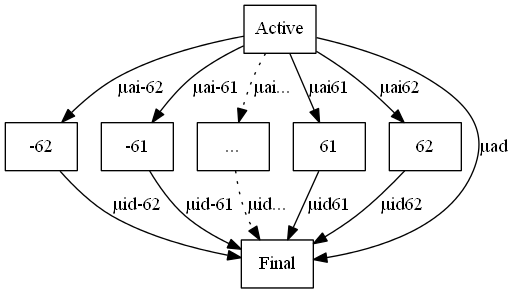
\includegraphics[scale=0.5]{gf820.png}
\caption{Markov-model for the parallelized GF820 Artificial Collective Spouse Pension plan.\label{fig:gf820}}
\end{figure}

The transition probability to one of the intermediary states $\mu_ai$ is the mortality intensity for the ensured at time $t + age$ times the marriage probability that a $t + age$ year old is married to a $t + age + diff$ year old where $diff$ is the number of the state.
The ensured to final state $mu_ad$ probability is the mortality intensity of the ensured at time $t + age$ times 1 minus the marriage probability at time $t + age$.
The intermediary to final state $mu_id$ probability is simply the mortality intensity of the spouse (assuming the sexuality of the ensured does not change) at age $t + age + diff$.

This does potentially lead to a lot of cases where the ensured will either be married to someone yet to be born or someone significantly older than the oldest person alive today, which is a problem for the Gompertz-Makeham mortality intensity methods.
To lessen the impact of this, the result of these functions are constrained to the range 0 to 1 by adding a constraint method during the AST conversion.

This model of calculation can already be expressed in CalcSpec as is, but is somewhat cumbersome to write as there is little variability in the model.
The final CalcSpec should resemble code sample \ref{gf820cs}.

\begin{lstlisting}[language=calcspec, caption=GF820 CalcSpec, label=gf820cs]
calculation = {
  name = "GF820 - Collective artificial spouse pension", 
  algorithm = { type = "Runge Kutta 4", parameters = { stepsize = 0.01 } }, 
  equations = { 
    0 = { r_j = rate, b_j = 0, mu_jk = { 
        1 = mu_ai(-62), 
        2 = mu_ai(-61), 
        ...,
        124 = mu_ai(61), 
        125 = mu_ai(62), 
        126 = \t.(GM_f(t + age)) * (1 - gp(t + age))
      }, b_jk = {  } }, 
    1 = { r_j = rate, b_j = 1, mu_jk = { 50 = mu_id(-62) }, b_jk = {  } }, 
    2 = { r_j = rate, b_j = 1, mu_jk = { 50 = mu_id(-61) }, b_jk = {  } }, 
    ...,
    124 = { r_j = rate, b_j = 1, mu_jk = { 50 = mu_id(61) }, b_jk = {  } }, 
    125 = { r_j = rate, b_j = 1, mu_jk = { 50 = mu_id(62) }, b_jk = {  } }, 
    126 = {  } }, 
  range = { from = 85, to = 0 }, 
  boundaryvalues = { 0 = 0, 1 = 0 }, 
  expressions = { 
    interestrate = 0.05, 
    age = 35, 
    rate(t) = interestrate, 
    GM_f(t) = constrain(0.0005 + 10 ^ (5.728 - 10 + 0.038 * (age + t))), 
    GM_m(t) = constrain(0.0005 + 10 ^ (5.88 - 10 + 0.038 * (age + t))), 
    mu_ai = \diff.\t.(GM_f(t + age)) * ((gp(t + age)) * (h(t + age + diff)(t + age))), 
    mu_id = \diff.\t.GM_m(t + age + diff) 
  }
}
\end{lstlisting}

To optimize this process, functionality was added to transform the CalcSpec AST based on the various variables of the GF820 plan.
See code sample \ref{gf820simplifiedcs} for an example of this.

\begin{lstlisting}[language=calcspec, caption=GF820 CalcSpec, label=gf820simplifiedcs]
calculation = { 
  name = "GF820 - Collective artificial spouse pension", 
  algorithm = { type = "Runge Kutta 4", parameters = { stepsize = 0.01 } }, 
  equations = { 
    GF820 = { age = age, rate = rate, mu_insured = GM_f, mu_spouse = GM_m }
  }, 
  range = { from = 85, to = 0 }, 
  boundaryvalues = { 0 = 0, 1 = 0 }, 
  expressions = { 
    interestrate = 0.05,
    age = 35,
    rate(t) = interestrate,
    GM_f(t) = constrain(0.0005 + (10 ^ (5.728 - 10 + 0.038 * (age + t)))),
    GM_m(t) = constrain(0.0005 + (10 ^ (5.88 - 10 + 0.038 * (age + t))))
  }
}
\end{lstlisting}

\subsubsection{Issues}
When attempting to compile the generated kernel with Alea.cuBase, an unexpected stack overflow exception was thrown.
By reducing the range of intermediary states from -62...+62 to 24 for double precision and 36 for single precision, it was able to be compiled again.
Various changes were made hoping to increase the number of intermediary states.
None were successful, but consisted of
\begin{itemize}
\item Reducing the depth of the generated AST by using a sum variable for the various state transitions
\item Reducing the local memory used by moving the temporary arrays to shared memory
\end{itemize}

More importantly, even with the mortality intensity functions constrained, the final results were not even close to matching the original results.
Whether this is an inherent problem with the parallelized version or there is something missing I do not know.
The results would be different given all 125 intermediary states, but it is very unlikely that they would align with the original results by just this.